\documentclass{suturo}

\begin{document}
    \maketitle{Vision}{13.05.2017}{}{1}{}{}{}{}

\makeatletter
\newcommand{\chapterauthor}[1]{%
  {\parindent0pt\vspace*{-47pt}%
  \linespread{2.2}\large\begin{flushright}von: #1\end{flushright}%
  \par\nobreak\vspace*{0pt}}
  \@afterheading%
}
\makeatother

\section*{Zielsetzung}
Das Ziel von Vision im zweiten Meilenstein ist das Erkennen und Segmentieren mehrerer Objekte in einer wahrgenommenen Szene. Diese Objekte sollen extrahiert werden und die Posen der einzelnen Cluster zur weiteren Verarbeitung übergeben werden. 

\section*{Probleme}
\subsection*{Segmentieren und Extrahieren von mehreren Objekten}
Die Objekte müssen klar von der restlichen wahrgenommenen Szene extrahiert und in einzelne Cluster aufgeteilt werden.\\
\textbf{Lösung}: Die Planare werden so lange segmentiert, bis nur noch eine Fläche (der Tisch) übrig ist. Es werden dann nur die Punkte oberhalb der Tischfläche extrahiert. Dann werden die Objekte mit einer euclidean cluster extraction voneinander getrennt und als einzelne Objekte zwischengespeichert.

\subsection*{Features zur Klassifizierung ermitteln}
Normal- und Farb-Features werden zur Klassifizierung der ermittelten Objekte benötigt. \\
\textbf{Lösung}: Bestimmung von VFH-Features und aufteilen von RGB-Daten in Achter-Bins.

\subsection*{Posen der Objekte bestimmen}
Für eine sinnvolle Greifpose müssen die Punkt im Koordinatensystem sowie Rotation und Translation der Objekte bestimmt werden. 
\textbf{Lösung}: Vision erhält von Knowledge die klassifizierten Labels und Nummern der Objekte, deren Pose dann mit einem Alignment-Algorithmus und einer Verfeinerung durch den Iterative Closest Point ermittelt werden.

\section*{Architektur und Funktion}
\chapterauthor{Tammo Wübbena, Update: Alexander Link}
Das Vision-Paket \footnote{im weiteren Verlauf auch Vision-Package, vision-node oder einfach Paket oder vision genannt} dient zur Akquirierung und Verarbeitung visueller Informationen durch die Kinect-Kamera des PR2-Roboters.

\begin{figure}[!htb]
        \center{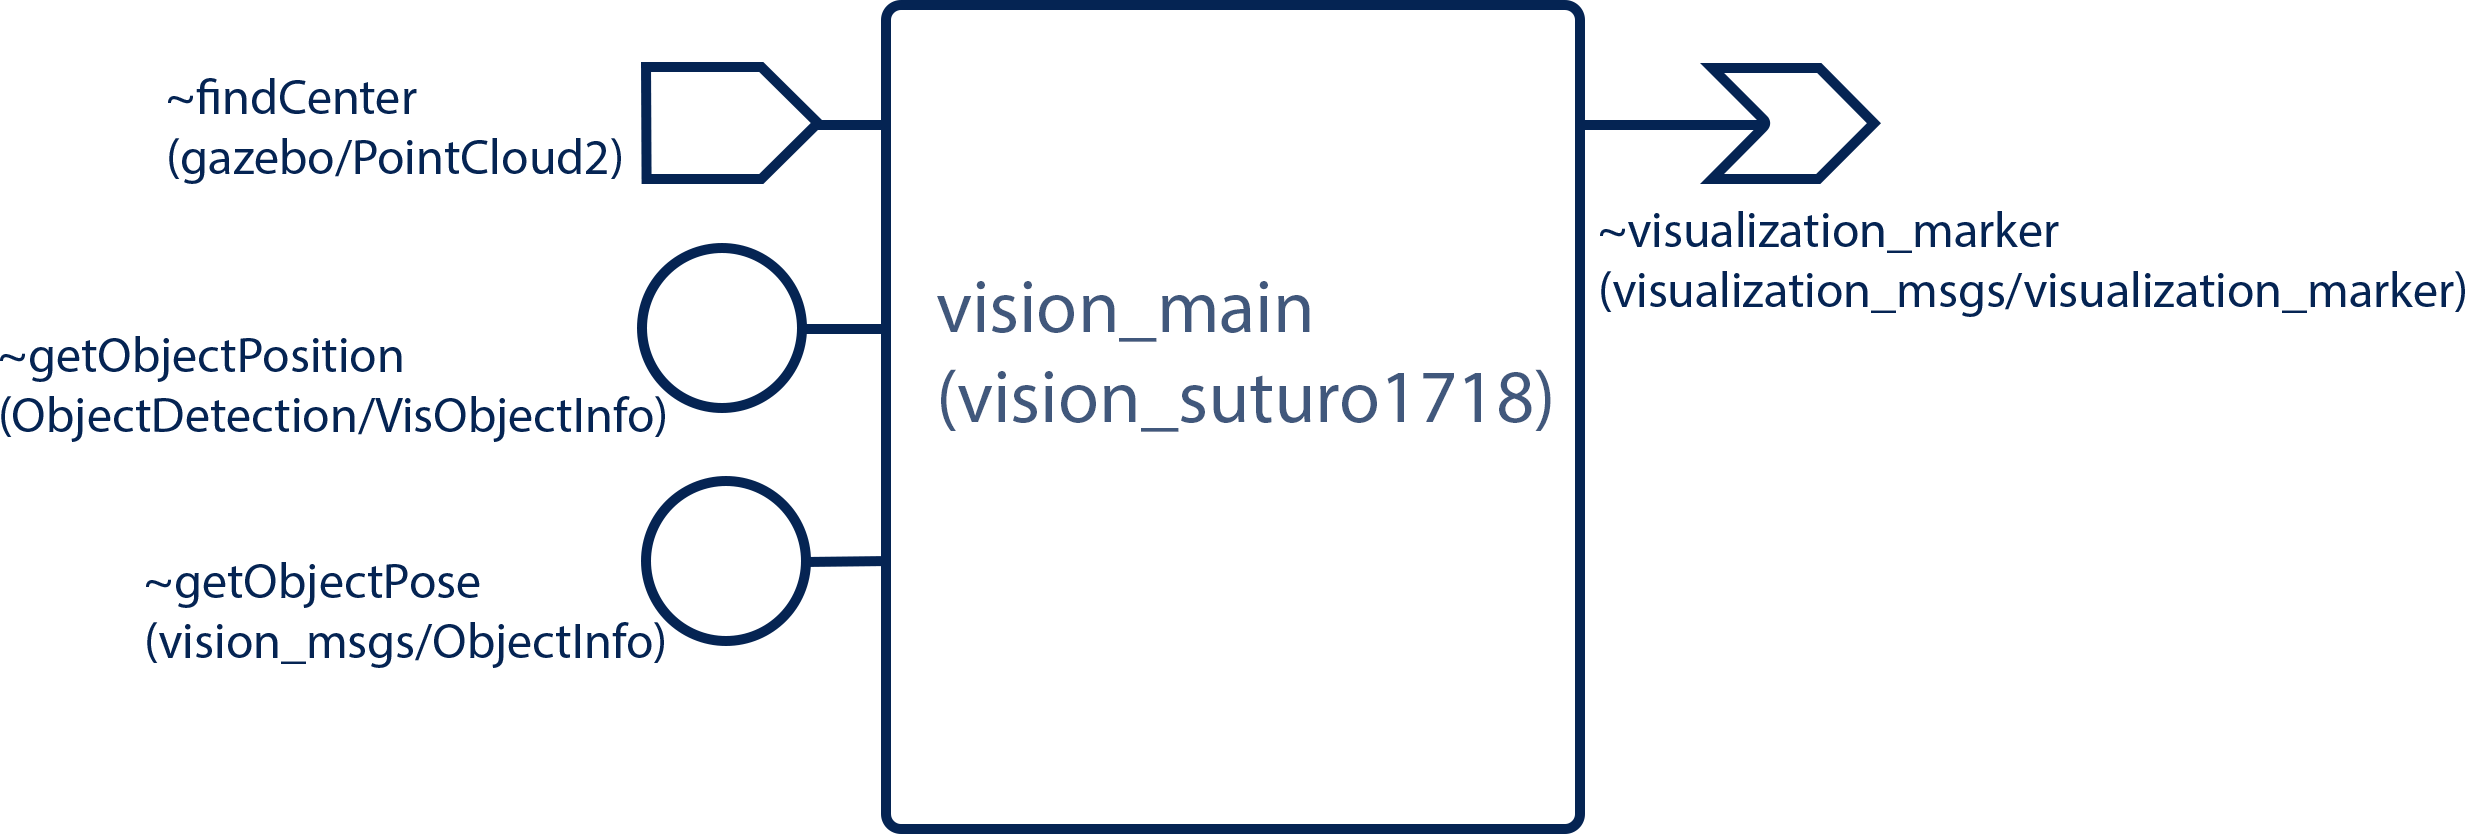
\includegraphics[width=\textwidth]
        {figures/vision_suturo_node_diagram_demo2.png}
        \caption{\label{fig:vision_node} Architektur der vision-node}}
\end{figure}
      
\section*{Methodendokumentation}
\chapterauthor{Tammo Wübbena}

\subsection{Abkürzungen durch short\_types.h}
Für bessere Lesbarkeit haben wir typedef Kürzel verwendet:
\begin{verbatim}
typedef pcl::PointCloud<pcl::PointXYZ>::Ptr PointCloudXYZPtr;
typedef pcl::PointCloud<pcl::PointXYZRGB>::Ptr PointCloudRGBPtr;
typedef pcl::PointCloud<pcl::Normal>::Ptr PointCloudNormalPtr;
typedef pcl::PointCloud<pcl::PointNormal>::Ptr PointCloudPointNormalPtr;
typedef pcl::PointCloud<pcl::PointXYZ> PointCloudXYZ;
typedef pcl::PointCloud<pcl::PointXYZRGB> PointCloudRGB;
typedef pcl::PointCloud<pcl::Normal> PointCloudNormal;
typedef pcl::PointIndices::Ptr PointIndices;
typedef std::vector<pcl::PointIndices> PointIndicesVector;
typedef std::vector<pcl::PointIndices::Ptr> PointIndicesVectorPtr;

typedef geometry_msgs::PointStamped PointStamped;
typedef pcl::PointCloud<pcl::VFHSignature308>::Ptr PointCloudVFHS308Ptr;
typedef sensor_msgs::PointCloud2 SMSGSPointCloud2;
typedef std::vector<pcl::PointCloud<pcl::PointXYZ>::Ptr> PointCloudXYZPtrVector;
\end{verbatim}

\subsection{Perception}

\subsubsection{preprocessCloud}
\begin{verbatim}
findCluster(const PointCloudXYZPtr kinect)
Beschreibung: Wendet unsere Filter auf eine Punktwolke an.
@param: kinect Punktwolke
@return: Vorprozessierte Punktwolke
\end{verbatim}\label{func:preprocesscloud}

\subsubsection{segmentPlanes}
\begin{verbatim}
void segmentPlanes(PointCloudRGBPtr cloud_cluster)
Beschreibung: Segmentiert Flächen, die nicht für die gesuchten Objekte relevant sind.
@param: PointCloud, aus der Flächen entfernt werden sollen.
\end{verbatim}\label{func:segmentplanes}

\subsubsection{findCluster}
\begin{verbatim}
std::vector<PointCloudRGBPtr> findCluster(PointCloudRGBPtr kinect)
Findet die Objekte und gibt eine Punktwolke pro Objekt zurück.
@param: Punktwolke der Kinect
@return: Punktwolken der Objekte
\end{verbatim}\label{func:findcluster}

\subsubsection{findCenterGazebo}
\begin{verbatim}
geometry_msgs::PointStamped findCenterGazebo()
Beschreibung: Gibt einen künstlichen Punkt zurück (Den Mittelpunkt des Modells, 
das an Gazebo übergeben wurde).
@return: Künstlicher 3D-Mittelpunkt
\end{verbatim}\label{func:findcentergazebo}


\subsubsection{findPoses}
\begin{verbatim}
std::vector<geometry_msgs::PoseStamped> findPoses(const std::vector<PointCloudRGBPtr> clouds_in)
Beschreibung: Errechnet Position und Rotation der Objekte in den übergebenen Punktwolken.
@param: Punktwolken der Objekte
@return: Posen der Objekte
\end{verbatim}\label{func:findposes}

\subsubsection{estimateSurfaceNormals}
\begin{verbatim}
PointCloudNormalPtr estimateSurfaceNormals(PointCloudRGBPtr input)
Beschreibung: Schätzt die Normalen einer Punktwolke.
@param: Punktwolke, zu der die Normalen berechnet werden sollen
@return: Normalen der übergebenen Punktwolke
\end{verbatim}\label{func:estimatesurfacenormals}

\subsubsection{apply3DFilter}
\begin{verbatim}
PointCloudRGBPtr apply3DFilter(PointCloudRGBPtr input, float x, float y, float z)
Beschreibung: Filtert eine Punktwolke, indem sie nur die Punkte in einem bestimmten
Bereich ((-x,x), (-y,y), (0.0,z)) erhält.
@param: Punktwolke, die gefiltert werden soll
		x,y,z Bereiche der Achsen für den Filter
@return Gefilterte Punktwolke
\end{verbatim}\label{func:apply3dfilter}

\subsubsection{estimatePlaneIndices}
\begin{verbatim}
PointIndices estimatePlaneIndices(PointCloudRGBPtr input)
Beschreibung: Errechnet die Indizes einer Fläche einer Punktwolke.
@param: Punktwolke, dessen Fläche ermittelt werden soll
@return Indizes der Fläche, wenn eine gefunden wurde
\end{verbatim}\label{func:estimateplaneindices}

\subsubsection{extractCluster}
\begin{verbatim}
PointCloudRGBPtr extractCluster(PointCloudRGBPtr input, PointIndices indices, 
bool negative);
Beschreibung: Extrahiert Objekt-Cluster anhand übergebener Punktwolke und Indizes.
@param: input Punktwolke, aus der ein Cluster extrahiert werden soll
		indices Indizes der Punkte in input, die extrahiert werden sollen
		negative Entscheidet, ob Indizes extrahiert werden sollen (false) oder
		alle Punkte, außer den in Indizes angegebenen (true).
@return Objekt-Cluster Punktwolke
\end{verbatim}\label{func:extractcluster}

\subsubsection{mlsFilter}
\begin{verbatim}
PointCloudRGBPtr mlsFilter(PointCloudXYZPtr input);
Beschreibung: Glättet Punktwolke unter Verwendung eines Moving-Least-Squares-Algorithmus.
@param: Punktwolke, die mittels MLS-Algorithmus geglättet wird
@return Geglättete Punktwolke
\end{verbatim}\label{func:mlsfilter}

\subsubsection{voxelGridFilter}
\begin{verbatim}
PointCloudRGBPtr voxelGridFilter(PointCloudRGBPtr input)
Beschreibung: Filtert eine Punktwolke mit dem Voxel-Gitter-Filter.
@param: Zu filternde Punktwolke
@return Mit einem Voxel-Gitter gefilterterte (und damit gedownsamplete) Punktwolke
\end{verbatim}\label{func:voxelgridfilter}

\subsubsection{outlierRemoval}
\begin{verbatim}
PointCloudRGBPtr outlierRemoval(PointCloudRGBPtr input)
Beschreibung: Entfernt Punkte aus Punktwolke, die als zu weit außen liegend
(outlier) oder als Rauschen erkannt werden.
@param: Punktwolke, die von Rauschen befreit werden soll
@return Gefilterte Punktwolke
\end{verbatim}\label{func:outlierremoval}

\subsubsection{cvfhRecognition}
\begin{verbatim}
PointCloudVFHS308Ptr cvfhRecognition(PointCloudRGBPtr input)
Beschreibung: Errechnet features eines Objekts in einer Punktwolke als VFHSignature308
@param: Punktwolke, dessen features berechnet werden sollen
@return Features als VFHSignature308
\end{verbatim}\label{func:cvfhRecognition}

\subsubsection{euclideanClusterExtraction}
\begin{verbatim}
std::vector<PointCloudRGBPtr> euclideanClusterExtraction(PointCloudRGBPtr input)
Beschreibung: Trennt cluster einer Punktwolke voneinander.
@param: Punktwolke
@return Eine Punktwolke pro cluster/Objekt
\end{verbatim}\label{func:euclideanClusterExtraction}

\subsubsection{SACInitialAlignment}
\begin{verbatim}
PointCloudRGBPtr SACInitialAlignment(std::vector<PointCloudRGBPtr> objects,
                                     std::vector<PointCloudVFHS308Ptr> features,
                                     PointCloudRGBPtr target)
Beschreibung: Errechnet Ausrichtung von Objekten bezüglich Zielen per sample consensus
@param: objects Punktwolken, features als VFHSignature308, target PointCloud
@return Punktwolke
\end{verbatim}\label{func:sacinitialalignment}

\subsubsection{iterativeClosestPoint}
\begin{verbatim}
PointCloudRGBPtr iterativeClosestPoint(PointCloudRGBPtr input,
                                       PointCloudRGBPtr target)
Beschreibung: Errechnet Ausrichtung eines Objekts zu einem Ziel anhand eines iterativen 
			  Closest-Point-Algorithmus.
@param: input Punktwolke, target Punktwolke
@return Punktwolke
\end{verbatim}\label{func:iterativeClosestPoint}

\subsubsection{produceColorHist}
\begin{verbatim}
std::vector<uint64_t> produceColorHist(pcl::PointCloud<pcl::PointXYZRGB>::Ptr  cloud)
Beschreibung: Errechnet ein Farbhistogramm einer Punktwolke.
@param: input Punktwolke eines Objekts, dessen Farbhistogramm errechnet werden soll
@return Farbhistogramm als floats (r,g,b)
\end{verbatim}\label{func:produceColorHist}

\subsubsection{getAllFeatures}
\begin{verbatim}
void getAllFeatures(std::vector<PointCloudRGBPtr> all_clusters, std::vector<float> vfhs_vector,
                    std::vector<uint64_t> color_features_vector)ud)
Beschreibung: Errechnet CVFH- und Farb-features für alle übergebenen Objekte.
@param: Punktwolken der Objekte, deren features errechnet werden sollen
\end{verbatim}\label{func:getallfeatures}

\subsubsection{getCVFHFeatures}
\begin{verbatim}
void getCVFHFeatures(std::vector<PointCloudRGBPtr> all_clusters, std::vector<float> current_features_vector)
Beschreibung: Errechnet CVFH-features von Punktwolken
@param: Punktwolken der Objekte, deren CVFH-features errechnet werden sollen
@return: CVFH features (Histogramme der Winkel zwischen einer zentralen viewpoint direction und jeder Normalen
\end{verbatim}\label{func:getcvfhfeatures}

\subsubsection{getColorFeatures}
\begin{verbatim}
void getColorFeatures(std::vector<PointCloudRGBPtr> all_clusters, std::vector<uint64_t> color_features_vector)
Beschreibung: Errechnet Farbfeatures von Punktwolken
@param: Punktwolken der Objekte, deren Farbfeatures errechnet werden sollen
	    Vektor für Farbfeatures, der befüllt wird
\end{verbatim}\label{func:getcolorfeatures}


\subsection{vision\_node}
\subsubsection{sub\_kinect\_callback}
\begin{verbatim}
void sub_kinect_callback(PointCloudRGBPtr kinect)
Beschreibung: Callback-Funktion für das kinect topic. Speichert die PointCloud ab,
sodass sie bereitsteht, wenn sie zur Prozessierung benötigt wird.
@param: Punktwolke des kinects
\end{verbatim}\label{func:subkinectcallback}
\subsubsection{start\_node}
\begin{verbatim}
void start_node(int argc, char **argv)
Beschreibung: Startet die Node zur Prozessierung von Punktwolken und der Kommunikation mit anderen Nodes.
@param: argc und argv ungenutzt
\end{verbatim}\label{func:startnode}
\subsubsection{getObjects}
\begin{verbatim}
bool getObjects(	vision_suturo_msgs::objects::Request &req, 
			    vision_suturo_msgs::objects::Response &res)
Beschreibung: Service zum Extrahieren von Objekten und deren Informationen aus einer Szene.
@param: req leere request, res Antwort mit den extrahierten Objekten nach ObjectsInfo.msg
@return true wenn service call erfolgreich, ansonsten false
\end{verbatim}\label{func:getobjects}


\subsection{CloudTransformer}

\subsubsection{extractAbovePlane}
\begin{verbatim}
PointCloudRGBPtr CloudTransformer::extractAbovePlane(PointCloudRGBPtr input)
Beschreibung: Findet die Hauptfläche (-> Tisch, etc.) und extrahiert nur die Punkte über dieser Fläche.
@param: Punktwolke
@return Extrahierte Punktwolke (ohne die Hauptfläche)
\end{verbatim}\label{func:extractaboveplane}
\subsubsection{transform}
\begin{verbatim}
PointCloudRGBPtr CloudTransformer::transform(const PointCloudRGBPtr cloud, std::string target_frame,
                 std::string source_frame)
Beschreibung: Transformiert eine Punktwolke in einen anderen frame.
@param: cloud Punktwolke, target_frame, source_frame
@return Transformierte Punktwolke
\end{verbatim}\label{func:transform}

\subsection{saving}
Hilfsfunktionen zum Speichern von Punktwolken als .PCD-Dateien.

\begin{verbatim}
void savePointCloudRGBNamed(pcl::PointCloud<pcl::PointXYZRGB>::Ptr cloud,
                            std::string filename);
void savePointCloudXYZ(pcl::PointCloud<pcl::PointXYZ>::Ptr cloud);
void savePointCloudXYZNamed(pcl::PointCloud<pcl::PointXYZ>::Ptr cloud, std::string filename);
void savePointCloudNormal(pcl::PointCloud<pcl::Normal>::Ptr cloud);
void savePointCloudPointNormal(pcl::PointCloud<pcl::PointNormal>::Ptr cloud);
void savePointCloud(pcl::PointCloud<pcl::PointXYZ>::Ptr objects,
                    pcl::PointCloud<pcl::PointXYZ>::Ptr kinect,
                    pcl::PointCloud<pcl::Normal>::Ptr normals);
\end{verbatim}

\subsection{viewer}
Hilfsfunktionen zur Darstellung von Punktwolken.
Enthält auch den momentan ungenutzten Visualization Marker.

\begin{verbatim}
void visualizePointCloud(pcl::PointCloud<pcl::PointXYZ> cloud);
void visualizeNormals(pcl::PointCloud<pcl::PointXYZ>::Ptr cloud, pcl::PointCloud<pcl::Normal>::ConstPtrnormals);
visualization_msgs::Marker publishVisualizationMarker(geometry_msgs::PointStamped point);
\end{verbatim}


\section*{Schnittstellen}
\chapterauthor{Alexander Link, Update: Tammo Wübbena}

\subsection*{Service Server /vision\_suturo/objects\_information}
\begin{verbatim}
objects.srv
@request: -
@response: ObjectsInfo msg (
							normal_features (VHFSignature308 as array)
							color_features (Color Histogram as array)
							object_amount (Number of objects in scene)
							object_poses (PoseStamped of objects in scene)
							object_information (additional information)
							object_errors (errors while extracting)
							)
\end{verbatim}
Gibt Anzahl, Features und Posen von den in einer Szene erkannten Objekten (Clustern) zurück. Die Pose wird für diesen Meilenstein noch nicht ermittelt. Der Service kann weitere Informationen und bei Problemen unterschiedliche Fehlermeldungen zurückgeben.
\\ \\
Die \textit{normal\_features} vom Typ VFHSignature308 und \textit{color\_features} (acht bins) aller Objekte werden konkateniert in Arrays festgehalten. 
Da die Länge der Features für ein Objekt immer gleich ist, kann durch die Anzahl der erkannten Objekte die Länge insgesamt ermittelt werden.

\subsection*{Subscriber REAL\_KINECT\_POINTS\_FRAME}
\begin{verbatim}
@response: PointCloudRGBPtr kinect
\end{verbatim}
Gibt eine Punktwolke unseres Sichtfelds (Szene oder Scene) zurück. Dabei wird auf das Topic \textit{/kinect\_head/depth\_registered/points} horcht. Alternativ kann mit \textit{SIM\_KINECT\_POINTS\_FRAME} auf \textit{/head\_mount\_kinect/depth\_registered/points} auf Simulationsdaten gehorcht werden.
\\ \\
Die Callback-Funktion wird im loop immer wieder aufgerufen, solange die Node noch aktiv ist bzw. der roscore-server besteht.

\subsection*{Service Client gazebo/get\_model\_state}
\begin{verbatim}
gazebo_msgs/GetModelState.srv
@request: -
@response:  string model_name,
            string relative_entity_name,
            std_msgs/Header header (uint32 seq, time stamp, string frame_id),
            geometry_msgs/Pose pose (...),
            geometry_msgs/Twist twist (...),
            bool success,
            string status_message
\end{verbatim}
Gibt Informationen über das gesuchte Objekt direkt aus gazebo aus.
\\ \\
Wird benutzt, um bei Problemen in der Simulation anstelle der vom kinect erkannten Daten auf die direkten Daten aus gazebo ausweichen zu können, an denen der Kinect-Sensor unbeteiligt ist.

\section*{Programmablauf}
\chapterauthor{Alexander Link, Update: Tammo Wübbena}
\subsection*{Schritt 1: Erkennen der Punktwolke}
Ein Subscriber empfängt die zu verarbeitenden Punktwolken des Kinect-Sensors und hält die wahrgenommene Szene aktuell.
\subsection*{Schritt 2: Service-Aufruf \textit{/vision\_suturo/objects\_information}}
Jedes mal, wenn der Service \textit{/vision\_suturo/objects\_information} durch Planning aufgerufen wird, wird die Funktion \textit{findCluster} in perception.h ausgeführt. 
\subsection*{Schritt 3: Vorbereiten auf die Extraktion} 
In \textit{findCluster} wird die Punktwolke zunächst folgendermaßen vorbearbeitet:

\begin{itemize} 
\item Ein PassThrough Filter, der den Sichtbereich begrenzt.
\item Ein VoxelGrid Filter zum Downsampling der eingehenden Punktwolke, indem für viele kleine 3-dimensionale Boxen der Mittelpunkte aller enthaltenden Punkte berechnet wird.
\item Ein MovingLeastSquares Filter, der Flächen begradigt, um Ungenauigkeiten der Daten vorzubeugen.
\item Das Entfernen von Flächen, die zu groß sind, um zum gesuchten Objekt gehören zu können. Dies passiert mehrmals, wenn es mehrere solcher Flächen im Sichtfeld gibt.
\end{itemize}
Eine Outlier-Removal wird nicht mehr benötigt, da die folgende Euclidean Cluster Extraction ''Ausreißer'', also weit von den Clustern entfernte Punkte nicht extrahiert.\\
\subsection*{Schritt 3b: Ausweichen auf Simulationsdaten}
Sollte es zu irgendeinem Zeitpunkt beim Filtern oder der Segmentierung zu Problemen kommen, weil beispielsweise die resultierende Punktwolke leer ist, wird auf die direkten Daten des Zielobjekts aus gazebo ausgewichen, wenn möglich.
\\
\subsection*{Schritt 4: Cluster Extraktion}
Mit \textit{EuclideanClusterExtracion} werden die nun segmentierten Objekte (alle noch in einer Punktwolke zusammengefasst) extrahiert und in einzelne Cluster gespeichert.
\\
\subsection*{Schritt 5: Berechnen von Features und Posen}
Es werden die Normal-Features, Color-Features für die Klassifikation durch Knowledge und die Posen der einzelnen Objekte berechnet.
 
\subsection*{Schritt 6: Befüllen der MSG}
Die einzelnen Features und Posen (letzteres aktuell noch nicht getestet) werden in der Message (ObjectsInfo.msg) gespeichert und zur weiteren Bearbeitung an Planning weitergegeben.

\subsection*{Visualization Marker}
Der Visualization Marker gibt den Mittelpunkt von Objekten aus. Dieser kann den anderen Gruppen beim debuggen helfen.

\section*{TODO: Zielsetzung, Probleme, Ausblick}
\chapterauthor{Tammo Wübbena}

\end{document}
